%% LyX 2.3.2-2 created this file.  For more info, see http://www.lyx.org/.
%% Do not edit unless you really know what you are doing.

\documentclass[onecolumn,floatfix,12pt]{revtex4-1}

\usepackage{hyperref}

\usepackage{fullpage}
\usepackage{graphicx}
\usepackage{wrapfig,framed}
\usepackage{xcolor}
\usepackage{braket}
\usepackage{amsmath}
\usepackage{tikz}
\usepackage{verbatim}
\usepackage{bookmark}
\usetikzlibrary{decorations.pathmorphing}
\usetikzlibrary{arrows}
\usepackage{nicefrac}

\newcommand{\lucas}[1]{\textbf{\textcolor{blue}{LKW: #1} } } 
\newcommand{\billy}[1]{\textcolor{red}{BP: #1}  } 
\newcommand{\filler}[1]{\textbf{\textcolor{magenta}{FILLER #1}}}
\newcommand{\vague}[1]{\textbf{\textcolor{green}{VAGUE #1}}}


\setcounter{secnumdepth}{3}
\usepackage{float}

\usepackage{babel}
\usepackage{comment} %Package to comment out regions.
\usepackage{biblatex} %Bibliography implementation package.
\renewcommand{\baselinestretch}{1.5} %Line spacing


\addbibresource{Prelim.bib}

\begin{document}


\title{Prelim document draft.}
\author{ Vasilios Passias \\ \underline {Advisor: }  Prof. Lucas K. Wagner}

\begin{abstract}
Abstract location.
\end{abstract}

\maketitle

\begin{comment}
Central Questions:  
\begin{itemize}
    \item Have we determined the existence of topological surface states (i.e. Fermi arcs)? 
    \item Have we found evidence for the oscillatory decay of Na$_3$Bi's band gap? Along which surface? 
    \item Is this demonstrated along other surfaces of Na$_3$Bi?
\end{itemize}

True statements:
\begin{itemize}
    \item 3D Dirac semimetals come in many forms.  
    \item The earliest example of a 3D Dirac semimetal was theoretically predicted and realized experimentally in BiTl(S$_{1-\delta}$ Se$_{\delta}$)$_2$ and (Bi$_{1-\delta}$In$_{\delta}$)$_{2}$ Se$_3$ as a phase transition between a trivial insulator and a 3D topological insulator.  
    \item Na$_3$Bi is a natural Dirac semimetal.
    \item It is a hexagonal crystalline system with a unit cell that contains 8 atoms. 6 of them are Na and 2 are Bi.
    \item This crystal has symmetries represented by the P$6_3$/mmc space group.
    \item In particular, this crystal has time-reversal and inversion symmetries as well as $C_3$ symmetry about the z-axis. 
    \item $C_3$ symmetry corresponds to 2 $\pi$/3 rotations about the z-axis. 
    \item Na$_3$Bi has two Dirac points on the rotation symmetry axis. 
    \item These Dirac points are formed from band inversion.
    \item The rotation symmetry that prevents the Dirac points from being gapped out is $C_3$ symmetry about the z-axis.
    \item Additionally, Na$_3$B has strong spin-orbit coupling.
    \item Near the Fermi level and around the $\Gamma$ point, the Na $3s$ orbitals comprise the conduction band while the valence band is composed of Bi $6p_x,p_y,p_z$ orbitals.
    \item Fermi arcs are surface states that connect the momentum space surface projections of the bulk Weyl points. 
    \item Fermi arcs are thought to exist on surfaces whose surface normals are not along the z-axis (along such surfaces, the Dirac points project onto a single Dirac point).
    \item Slabs of Na$_3$Bi exhibit band gap oscillations that decay with slab thickness.  
\end{itemize}

\end{comment}

\section{Introduce Gaps in Knowledge.}

\subsection{Density Functional Theory}

Describing solid state systems requires dealing with a large number of electrons and ions.  In order to describe such a system we need to solve the many-particle Schrodinger equation involving a many-particle wavefunction:

\begin{align}
i\hbar\frac{\partial \psi(\{\textbf{r}_e\},\{\textbf{r}_A\};t)}{\partial t} = \hat{H} \psi(\{\textbf{r}_e\},\{\textbf{r}_A\};t) \label{eq:1} \\
\hat{H} = - \sum_{i}^{N} \frac{\hbar^{2}}{2m} \nabla^{2}_{i} - \sum_{I}^{N_{I}} \frac{\hbar^{2}}{2 M_{I}} \nabla^{2}_{I} - \sum_{i}^{N} \sum_{I}^{N_{I}} \frac{Z_{I}e^2}{|r_i - R_I|} + \sum_{i < j} \frac{e^2}{|r_{i} - r_{j}|} + \sum_{I < J }^{N_{I}} \frac{Z_{I} Z_{I} e^2 }{|R_{I} - R_{J}|}
\label{eq:2}
\end{align}

\noindent In equation (\ref{eq:1}) the many-particle wavefunction accounts for the electrons and nuclei.  The positions of the electrons and nuclei are noted in that equation by $\{\textbf{r}_e\}$ and $\{\textbf{r}_A\}$, respectively.  The Hamiltonian of this system is shown in equation (\ref{eq:2}). Electrons are associated with the indices $i$ and $j$, while nucleons are associated with the indices $I$ and $J$.  Equation (\ref{eq:1}) is very difficult to solve in practice given the large number of electrons and ions in a solid, but we can use an approximation to make the problem easier.  One approximation is given that the nuclei are more massive than the electrons, the former's motion can be neglected.  This simplification is at the heart of the Born-Oppenheimer approximation. Consequently, we can focus on the electronic part of the Hamiltonian and wavefunction:  

\begin{align}
    \hat{H}_{e} = - \sum_{i}^{N} \frac{\hbar^{2}}{2m} \nabla^{2}_{i} - \sum_{i}^{N} \sum_{I}^{N_{I}} \frac{Z_{I}e^2}{|r_i - R_I|} + \sum_{i < k} \frac{e^2}{|r_{i} - r_{k}|} + \sum_{I < J }^{N_{I}} \frac{Z_{I} Z_{I} e^2 }{|R_{I} - R_{J}|}\label{eq:3} \\
    \hat{H}_{e}\psi(\textbf{r}_1,\cdots,\textbf{r}_N) = E_{e} \psi(\textbf{r}_1,\cdots,\textbf{r}_N) \label{Electron_eval}
\end{align}

\noindent The last term in equation (\ref{eq:3}), which corresponds to the Coulomb interaction between nuclei, can be regarded as a constant shift in the energy. Although we have simplified the problem, solving for the electron eigenenergies in equation (\ref{Electron_eval}) still remains a daunting task for a large number of electrons in a typical crystalline solid. 

We can approach the eigenvalue problem in equation (\ref{Electron_eval}) in a different via multiplying both sides by $\psi(\textbf{r}_1,\cdots,\textbf{r}_N)$ and subsequently integrate over all electronic positions: 

\begin{align}
    \int \psi^{*}(\textbf{r}_1,\cdots,\textbf{r}_N)\hat{H}_{e}\psi(\textbf{r}_1,\cdots,\textbf{r}_N) d\textbf{r}_1 \cdots d\textbf{r}_N = E_{e} \int \psi^{*}(\textbf{r}_1,\cdots,\textbf{r}_N) \psi(\textbf{r}_1,\cdots,\textbf{r}_N) d\textbf{r}_1 \cdots d\textbf{r}_N  \\
    E_{e} = \frac{\int \psi^{*}(\textbf{r}_1,\cdots,\textbf{r}_N)\hat{H}_{e}\psi(\textbf{r}_1,\cdots,\textbf{r}_N) d\textbf{r}_1 \cdots d\textbf{r}_N}{\int \psi^{*}(\textbf{r}_1,\cdots,\textbf{r}_N) \psi(\textbf{r}_1,\cdots,\textbf{r}_N) d\textbf{r}_1 \cdots d\textbf{r}_N} \label{E_energy}
\end{align}

\noindent We see that the electron energy can be written as a functional of the electronic wavefunction.  Given the normalization requirement of the wavefunction, the denominator of equation (\ref{E_energy}) is unity.     

\subsection{Topological Insulators}

Topological materials have garnered significant attention in the condensed matter community in past few years because of their peculiar electronic properties. There are non-interacting and strongly interacting topological systems.\cite{hasan_colloquium:_2010,qi_topological_2011,rachel_interacting_2018} Here we will focus on topological Dirac semimetals which are non-interacting electronic topological systems related to topological insulators.  Let us first discuss what topological insulators are. 

Topological insulators feature an insulating (or gapped) band spectrum in the volume of the material.  What this gapped spectrum means is the filled valence and the empty conduction bands are separated by a finite energy difference that cannot be surmounted by electrons at room temperature. The gapped spectrum is a discontinuity between the filled states and the empty states. Although the bulk is insulating, the surface enclosing the bulk possesses conducting (or gapless) states. These gapless states are termed chiral currents, which are characterized by spin-momentum locking. Effectively, the propagation direction of the charge carriers is set by their spin degree of freedom. These surface states cross the bulk band gap and connect the bulk valence and conduction bands. At energies and momenta near the surface band crossing points, the dispersion attains a non-relativistic massless Dirac dispersion relation. The chiral surface states are "protected" from being gapped, for sufficiently thick samples so as to prevent the hybridization and subsequent gapping of opposite moving chiral states, as long as time-reversal symmetry is preserved. Topological insulators are not simply a theoretical construct.  A number of materials like HgTe quantum well structures, an example of a 2D topological insulator, and BiSe$_3$, a 3D topological insulator, have been discovered that demonstrate chiral surface currents and an insulating bulk.\cite{konig_quantum_2007,zhang_topological_2009} 

\subsection{Introducing Weyl and Dirac semimetals.}

Since the theoretical prediction and subsequent experimental discovery of topological insulators, new materials which feature both a gapless bulk and surface states have been theroetically proposed and experimentally verified. These materials are known as topological semimetals.\cite{noauthor_topological_nodate} There are a variety of topological semimetals like Weyl, Dirac, and nodal line semimetals, just to name a few.  We will look at Weyl and Dirac semimetals because they share a number of common traits, but also important differences. Part of this is based on the type of degeneracies in the band plots. We will provide a short explanation about their differences.

In a band structure plot of the energy states bands corresponding to different energy eigenvalues can form degenerate points from accidental degeneracies (i.e. from tuning parameters in the Hamiltonian such that two or more energy levels can have the same energy). The presence of symmetries can increase the degeneracy of the band crossing points. (There are symmetries that can induce band crossings?) Most of the 3-D semimetals have time reversal and inversion symmetries. Inversion symmetry reverses the sign of the momentum, but not the spin of the particular band:

\begin{equation}
E_{n,\sigma}\left({\bf k}\right)=E_{n,\sigma}\left(-{\bf k}\right).
\end{equation}

\noindent Time reversal symmetry reverses both the spin of the particular band and the sign of the momentum:

\begin{equation}
E_{n,\uparrow}\left({\bf k}\right)=E_{n,\downarrow}\left(-{\bf k}\right).
\end{equation}

\noindent If both time-reversal symmetry and inversion symmetry are present, then:

\begin{equation}
E_{n,\uparrow}\left({\bf k}\right)=E_{n,\downarrow}\left({\bf k}\right),
\end{equation}

\noindent which indicates that there is a double degeneracy for bands of different spin components at each k-point. If there is a degeneracy of bands, at some momentum ${\bf k}_{0}$, of different quantum number $n$, say $n$ and $n+1$, then that band crossing point is four-fold degenerate.  If we expand the Hamiltonian for momenta near the band crossing point and if the result gives a gapless dispersion relation that is linear with momentum,  then this band crossing point can be regarded as an emergent  non-relativistic Dirac particle. In the case where there is a breaking of time-reversal symmetry, or inversion-symmetry, or both, the double degeneracy of the a single band is lifted over generic points in the Brillouin zone. When two such bands meet at the same energy at some momentum in the Brillouin zone, there is a degeneracy of two. If one expands the Hamiltonian around the momentum crossing point of the two bands, and if one finds a non-relativistic Weyl dispersion, such band crossings are called Weyl nodes. Each Weyl node carries a non-zero ``charge'' which is computed by integrating the Berry curvature, $\vec{\Omega}_{n}(\bf{k})$, around a small closed surface $S$ that encloses the Weyl node.  This is defined as the Chern number:

\begin{eqnarray}
C = \frac{1}{2\pi} \sum_{n=1}^{n=N} \oint_S \vec{\Omega}_{n}(\text{k}) \cdot d\vec{S}_{\vec{k}}\\
\vec{\Omega}_{n}(\bf{k}) = \nabla_{\bf{k}} \times -i \langle u_n (\bf{k}) |  \nabla_{\bf{k}} |u_n (\bf{k})\rangle
\end{eqnarray}

\noindent $|u_n(\bf{k})\rangle$ is the Bloch wavefunction. Here we assume there are $N$ filled bands.   

Weyl semimetals have a bulk momentum space that is characterized by an even number of band crossing points where two non-degenerate bands meet. The total Chern number of all the Weyl points in the bulk momentum space is zero, which indicates that there are equal number of Weyl points with opposite Chern number in the bulk Brillouin zone.  These degeneracies are stable as long as they remain at different momenta.  If the Weyl points of opposite Chern number coincide in momentum space, the degenercy of the two states is lifted and one finds a finite energy gap.  The degeneracies in the bulk momentum space of the Weyl semimetal have interesting surface states that appear on the surface Brillouin zone of the Weyl semimetal. These surface states are known as Fermi arcs which are incomplete Fermi surfaces that connect the surface projections of the bulk Weyl points on opposite surfaces.  

For Dirac semimetals the Dirac point is a four-fold degenerate point in momentum space.  This point has a vanishing net Chern number since it contains two Weyl points of opposite Chern number. Certain symmetries are needed required in order for the Dirac point to remain stable at the same momentum space point.  At first, the existence of a Dirac semimetal was thought to exist at the phase boundary between a topological insulator and a conventional insulator, as long as time reversal and inversion symmetry were preserved, thereby giving a four-fold degenerate bulk band crossing at the phase boundary \cite{noauthor_topological_nodate}.  
A material that exhibits this property was theoretically predicted and realized experimentally in BiTl(S$_{1-\delta}$ Se$_{\delta}$)$_2$ and (Bi$_{1-\delta}$In$_{\delta}$)$_{2}$ Se$_3$ \cite{xu_topological_2011,brahlek_topological-metal_2012}.  However, there have since been other realizations of topological Dirac semimetals.   

\subsection{Gaps in knowledge: Existence of Fermi arcs in Na$_{3}$Bi.}

In our studies, we look at Na$_{3}$Bi, which is a theoretically and experimentally realized natural topological Dirac semimetal, in that it does not arise at a phase transition between a trivial insulator and a topological insulator\cite{wang_dirac_2012,liu_discovery_2014}.  Na$_{3}$Bi is a hexagonal crystalline system with a unit cell that contains 8 atoms, 6 of them are Sodium (Na) atoms and 2 are Bismuth (Bi) atoms\cite{wang_dirac_2012}.  This crystal has strong spin-orbit coupling along with time-reversal and inversion symmetries as well as symmetries represented by the P$6_3$/mmc space group. In particular, the crystal has $C_3$ symmetry about the z-axis. $C_3$ symmetry corresponds to 2 $\pi$/3 rotations about the z-axis. It is this symmetry that prevents the Dirac points from being gapped out. Na$_3$Bi has two Dirac points on the z-axis. These Dirac points are formed in the bulk from band inversion\cite{yang_classification_2014}.  Near the Fermi level and around the $\Gamma$ point, the Na $3s$ orbitals comprise the conduction band while the valence band is composed of Bi $6p_x,p_y,p_z$ orbitals.(citation needed). The effective Hamiltonian $H(\textbf{k})$ near the $\Gamma$ point is:

\begin{eqnarray}\label{H_effective}
H(\textbf{k}) = \epsilon_{0}(\textbf{k})I^{4\times4}_{0} +
\begin{bmatrix}
M(\textbf{k}) & \lambda k_{+} & 0 & 0 \\
\lambda k_{-} & -M(\textbf{k}) & 0 & 0 \\
0 & 0 & M(\textbf{k}) & -\lambda k_{-} \\
0 & 0 & -\lambda k_{+} & -M(\textbf{k})
\end{bmatrix}
\end{eqnarray}

\noindent Here $\epsilon_{0}(\textbf{k})$ is some momentum dependent offset energy, $k_{\pm} = k_{x} \pm k_{y}$, and $M(\textbf{k}) = M_{0} - M_{1}k^2_{z} - M_{2}(k^2_{x} + k^2_{y})$. $I^{4\times4}_{0}$ denotes the $4 \times 4$ identity matrix. This Hamiltonian is written in the basis of $| S_{J=\frac{1}{2}},J_{z} = \frac{1}{2}  \rangle$, $| P_{J=\frac{3}{2}},J_{z} = \frac{3}{2}  \rangle$,
$| S_{J=\frac{1}{2}},J_{z} = -\frac{1}{2}  \rangle$,
and $| P_{J=\frac{3}{2}},J_{z} = -\frac{3}{2}  \rangle$.  After diagonalizing equation (\ref{H_effective}) we find the energy eigenvalues are:

\begin{eqnarray}\label{E_pm}
E_{\pm}(\textbf{k}) =\epsilon_{0}(\textbf{k}) \pm \sqrt{A^2 k_{+} k_{-}   + (- M_{0} + k^2_{z} M_{1} + M_{2} k_{+} k_{-} )^2}
\end{eqnarray}

\noindent Clearly, the energy difference between the two energy eigenvalues vanishes if the term in the square root is zero.  It can occur for two momenta $\textbf{k}^{D}_{\pm} = ( 0, 0, \pm \sqrt{M_{0}/M_{1}} )$, which are the locations of the Dirac points along the $z$-axis. Since there are two Weyl points per Dirac node, there should be twice as many Fermi arcs on the surfaces of a Dirac semimetal. However, not all surfaces have Fermi arcs; they exist on surfaces whose surface normals are not along the z-axis (along such surfaces, the Dirac points project onto a single Dirac point). Surfaces orthogonal to the axis containing the Dirac points will instead have a Dirac point crossing at that surface in the band plot.


\subsection{Gaps in knowledge: band gap oscillations in Na$_{3}$Bi?}

One interesting observation made by the authors of \cite{xiao_anisotropic_2015} is the effect of confinement on the band gap of Na$_{3}$Bi.  By confinement we mean the direction in which Na$_{3}$Bi has open boundary conditions, or the direction in which layers of this crystal are added.  Since the low energy physics of Na$_{3}$Bi has emergent Dirac physics near the $\Gamma$ point of the Brillouin zone, it is evident that the emergent Dirac quasiparticles have a long wavelength, since their wavenumbers are inversely related to their wavelengths.  Therefore, confining the structure along any direction should affect these quasiparticles, and, hence, the band plots in which they are observed. The authors study such effects using a tight-binding model Hamiltonian of the following form:


\begin{eqnarray}
H_{lattice} = \sum_{i,j,k} V_{i,j,k} c^{\dagger}_{i,j,k}c_{i,j,k} 
+ \sum_{i,j,k} \left( T_{x} c^{\dagger}_{i+1,j,k}c_{i,j,k} +T_{y} c^{\dagger}_{i,j+1,k}c_{i,j,k} +T_{z} c^{\dagger}_{i,j,k+1}c_{i,j,k} + H .c. \right) 
\end{eqnarray}

Here $c^{\dagger}_{i,j,k}$ and $c_{i,j,k}$ are creation and destruction operators for site $(i,j,k)$. $T_x$, $T_y$, $T_z$ are nearest neighbor hopping matrix elements. The authors used a 3D tetragonal lattice with lattice parameters $a_x = a_y = 0.3$ nm,  $a_z = 0.5$  nm. There were 2 confinement directions: along $y$ and along $z$.  The confinement direction along $y$ exhibited a decay in the band gap that went as $1/W_y$, where $W_y$ denotes the thickness of the slab along the y-direction. However, if the structure is confined along the $z$-direction, the authors find the band gap exhibits oscillations that decay with slab thickness. We propose to verify these results using density functional theory with spin-orbit coupling.

\section{Demonstration of research done.}


%Fermi arcs in the Na3Bi (110) plane.
\subsection{Investigating the existence of Fermi arcs in the Na$_{3}$Bi (110) plane.}

We investigated whether or not the Fermi arc surface states of Na$_{3}$Bi exist on the (110) direction, or more accurately the (11$\bar{2}$0) direction, since we are dealing with a hexagonal lattice. We chose this direction because this surface is parallel to the $k_{z}$ axis along which there are two Dirac point crossings.  It is believed the Fermi arc surface states appear on this surface for $k_{z}=0$ since this momentum is time-reversal symmetric \cite{kargarian_are_2016}. However, it's not clear if such surface states exist, since terms that respect the symmetries of Na$_{3}$Bi and do not gap out the bulk Dirac points can gap out the Fermi arc surface states\cite{kargarian_are_2016}.  Given that a previous study \cite{xu_observation_2015} has confirmed the existence of Fermi arcs along the (100) direction, we attempted to reproduce the findings in order to give us an intuition about the signatures of such surface states.  

\begin{figure}[H]
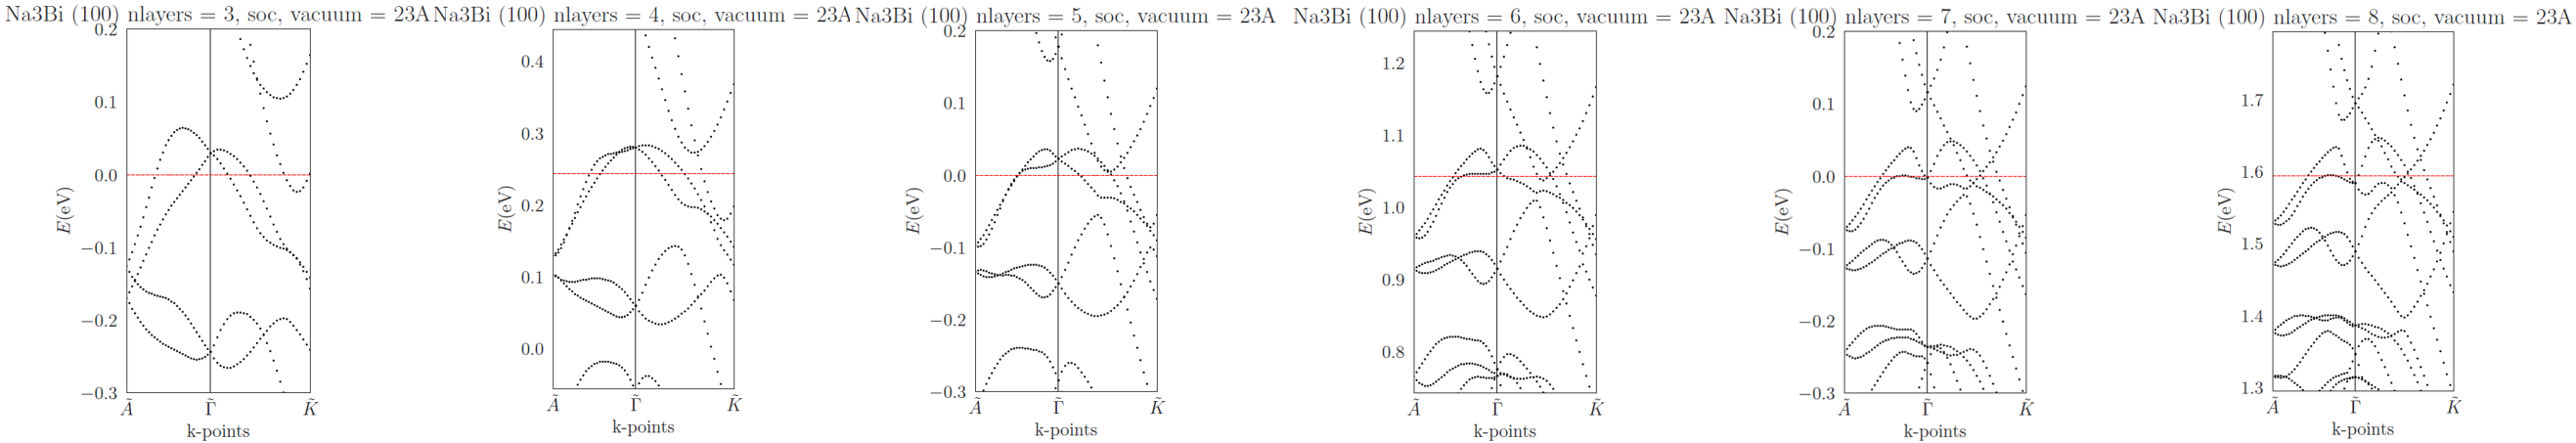
\includegraphics[scale=0.40]{Na3Bi_100_nlayer_var_vac23A.png}\caption{\label{fig:Na3Bi_100_var_nlayers_vac23A} Band plots for a 23 A vacuum surrounding a varying number of Na$_3$Bi (100) layers. The red line is the Fermi level.}
\end{figure}

We see in Figure \ref{fig:Na3Bi_100_var_nlayers_vac23A} the number of bands increases as we increase the number of layers orthogonal to the (100) direction.  We should expect to see a bulk Dirac point emerge between the k-points $\tilde{A}$ and $\tilde{\Gamma}$.   However, we need thicker structures in order to see this Dirac point. We are also unable to distinguish the Fermi arc surface states from the bulk states, which requires thicker structures beyond 12 layers, along with possible relaxations in the crystal geometry.  

\subsection{Na$_{3}$Bi (110) slab and vacuum thickness effects on Na$_{3}$Bi's band structure.}

\begin{figure}[H]
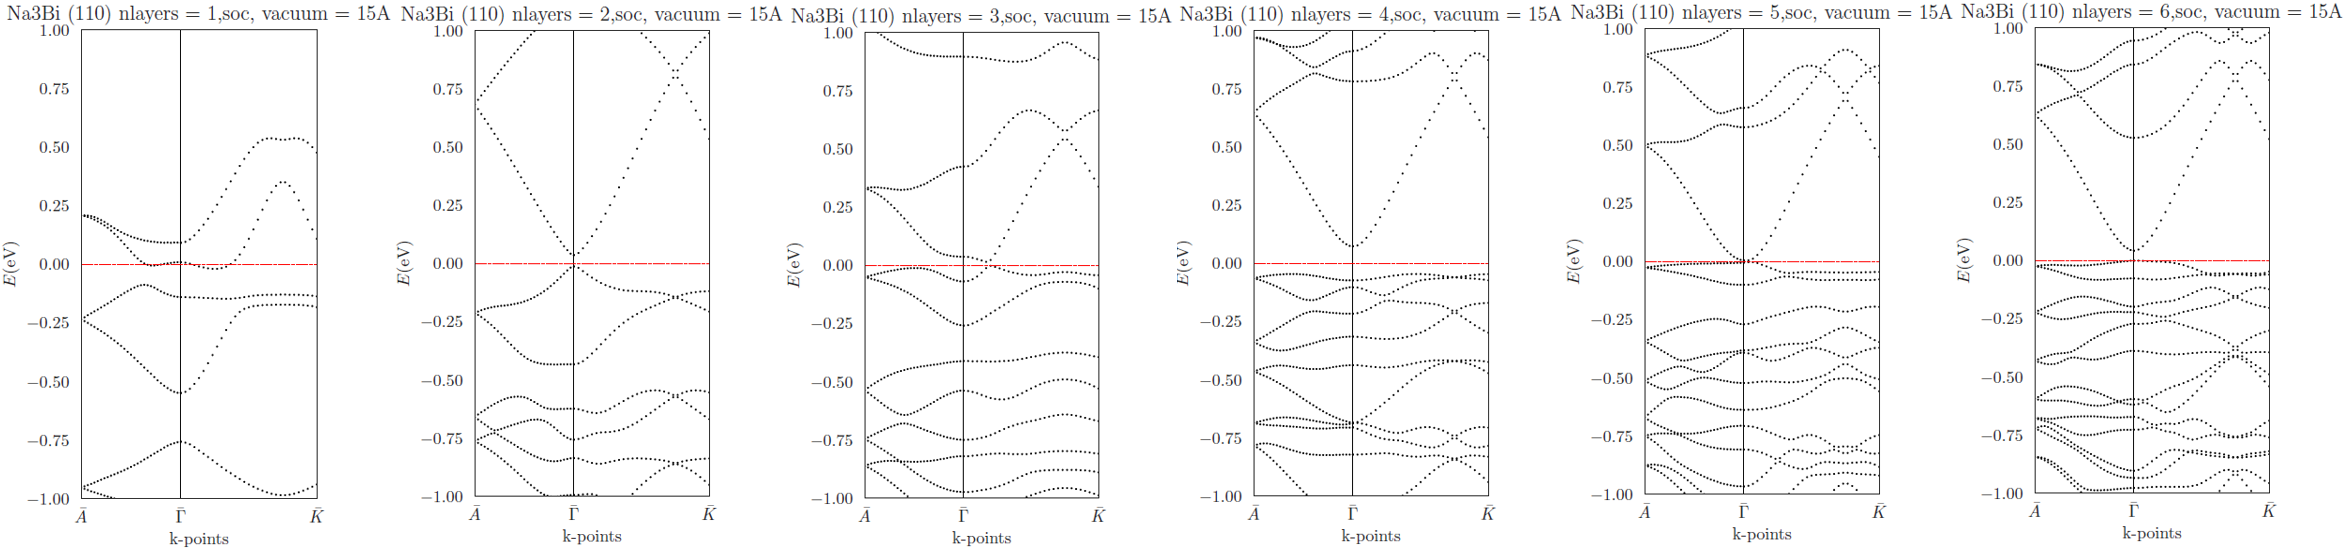
\includegraphics[scale=0.4]{Na3Bi_110_var_nlayers_vac15A.png}\caption{\label{fig:Na3Bi_110_var_nlayers_vac15A}Band plots of the Na$_{3}$Bi (110) system with fixed vacuum thickness but varying system thickness. The red line is the Fermi level.}
\end{figure}

Figure \ref{fig:Na3Bi_110_var_nlayers_vac15A} demonstrates that as the number of Na$_{3}$Bi layers increases, the band gap size at the $\bar{\Gamma}$ point oscillates. Odd number of layers have a smaller band gap than even number of layers. This is consistent with the observed oscillatory decay of Na$_{3}$Bi's band gap when the confining direction (i.e. the direction with open boundary conditions) is along the z-direction \cite{xiao_anisotropic_2015}. Overall the oscillating band gap of the (110) layers is in contrast to what is seen in Figure \ref{fig:Na3Bi_100_var_nlayers_vac23A} for the (100) direction.  



\begin{comment}
%Na3Bi band gap oscillations.
\subsection{Na$_{3}$Bi (110) slab and vacuum thickness effects on Na$_{3}$Bi's band structure.}

\begin{figure}[H]
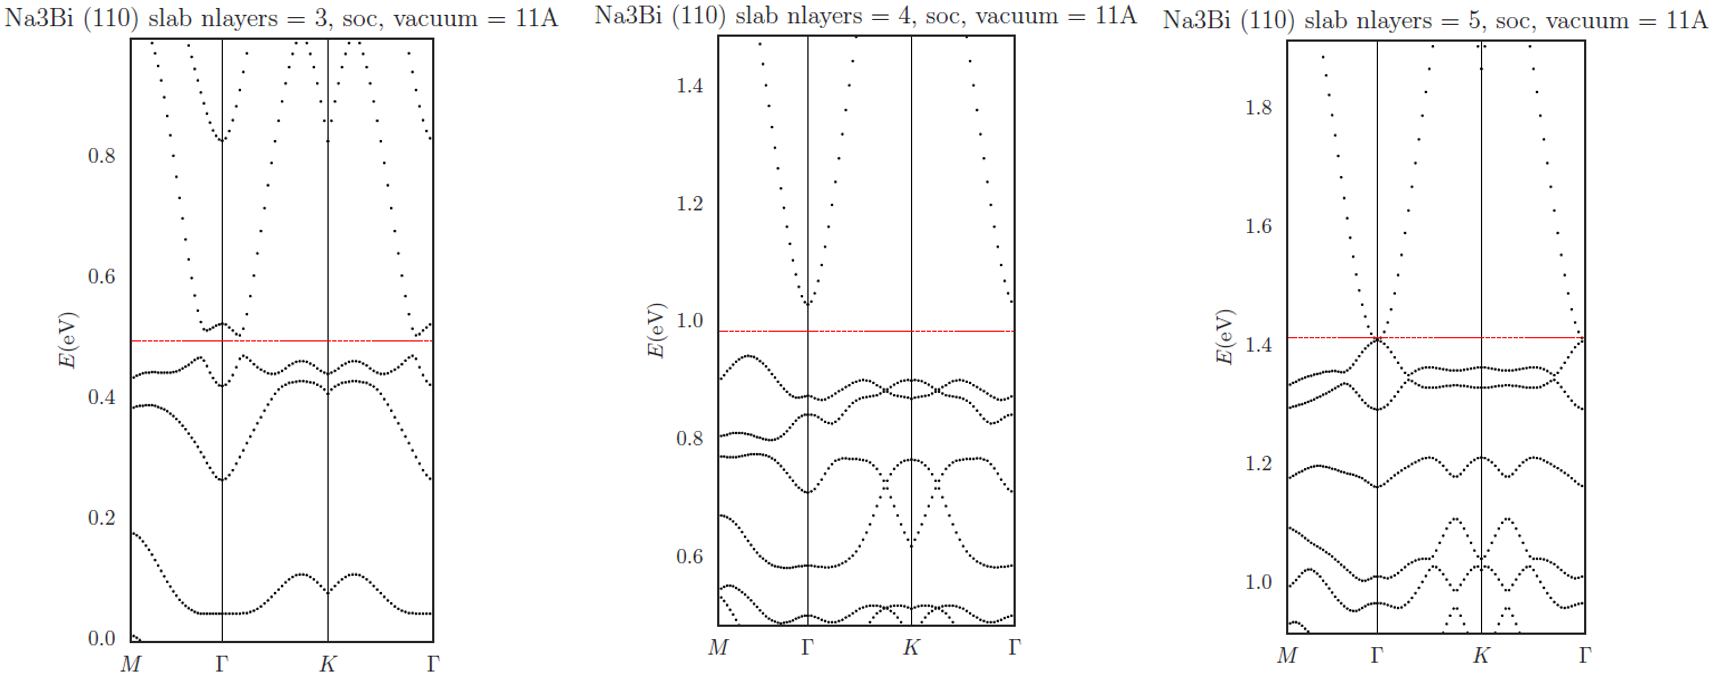
\includegraphics[scale=0.62]{Na3Bi_change_nlayers_vac_11A}\caption{\label{fig:Band-plots-of Na3Bi changing thickness}Band plots of the
Na$_{3}$Bi (110) system with fixed vacuum thickness but varying system thickness. The red line is the Fermi level.}
\end{figure}

We see in Figure \ref{fig:Band-plots-of Na3Bi changing thickness} that as the number of Na$_{3}$Bi layers increases, the band gap size at the $\Gamma$ point oscillates. Odd number of layers have a smaller band gap than even number of layers. This is consistent with the oscillatory decay of Na$_{3}$Bi's band gap when the confining direction (i.e. the direction with open boundary conditions) is along the z-direction. We are interested in what happens near the $\Gamma$ point because that is where the low energy physics is usually observed and also because at that momentum, the band inversion is most visible. We see hints of the band inversion for the 3 layer Na$_{3}$Bi (110) structure above at the $\Gamma$ point, for the conduction and valence bands nearest the Fermi level.

The oscillatory decay of Na$_{3}$Bi's band gap is not found in all cuts of Na$_{3}$Bi.  For example the (100) surface does not appear to exhibit this behavior.  


\begin{figure}[H]
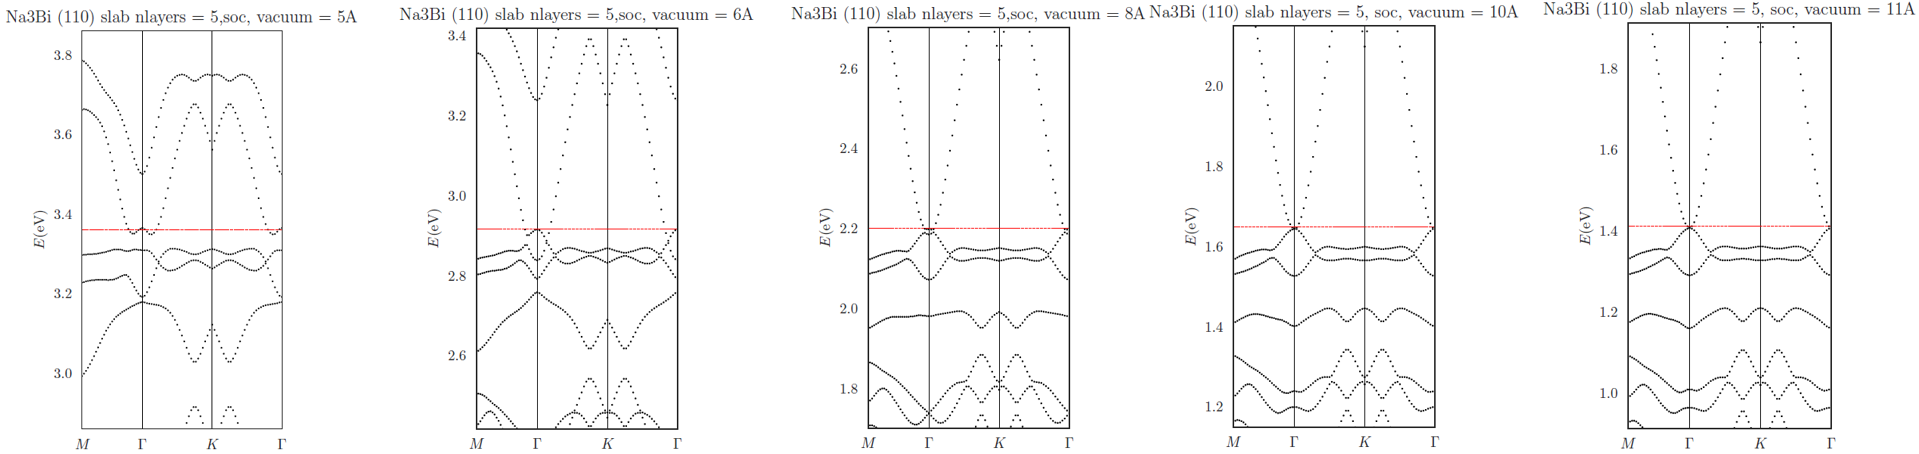
\includegraphics[scale=0.6]{Na3Bi_nlayer_5_change_vac}\caption{\label{fig:Na3Bi Fixed odd number layers incr vac}Band plots for a variable vacuum thickness surrounding a 5 layer Na$_3$Bi structure.}
\end{figure}

Figure \ref{fig:Na3Bi Fixed odd number layers incr vac} summarizes how changing the vacuum thickness affects the band plots of a 5 layer Na$_3$Bi system. We find hints of band inversion for bands nearest the Fermi level at the $\Gamma$ point for the system surrounded by an 8A vacuum layer. Overall the band plots demonstrate little to no band gaps around the Fermi level near the $\Gamma$ point.


\begin{figure}[H]
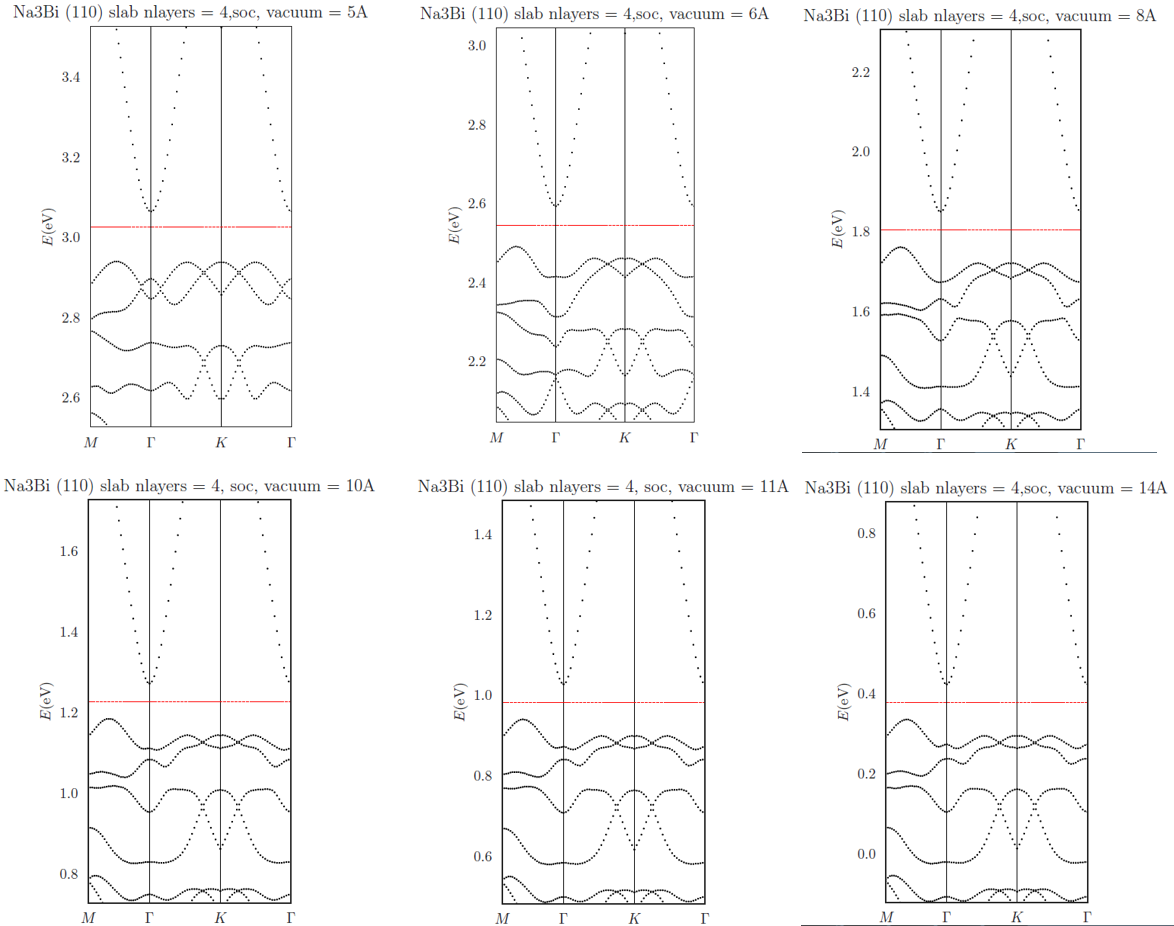
\includegraphics[scale=0.65]{Na3Bi_nlayer4_change_vac}

\caption{\label{fig:Na3Bi Fixed even number layers incr vac} Band plots for a variable vacuum thickness surrounding a 4 layer Na$_3$Bi structure.}
\end{figure}

If we compare Figure \ref{fig:Na3Bi Fixed even number layers incr vac} with Figure \ref{fig:Na3Bi Fixed odd number layers incr vac} we observe a larger band gap in the former than the latter for similar vacuum thicknesses. There does not appear to be any band inversion in the character of the bands nearest to the Fermi level at the $\Gamma$ point.  Overall, we need to find the Berry curvature of these systems in order to definitively determine their topological characteristics.



%Fat band calculations for plain Na3Bi.
\subsection{Contributions of Na and Bi atom orbitals to the Na$_{3}$Bi band plots.}

\begin{figure}[H]
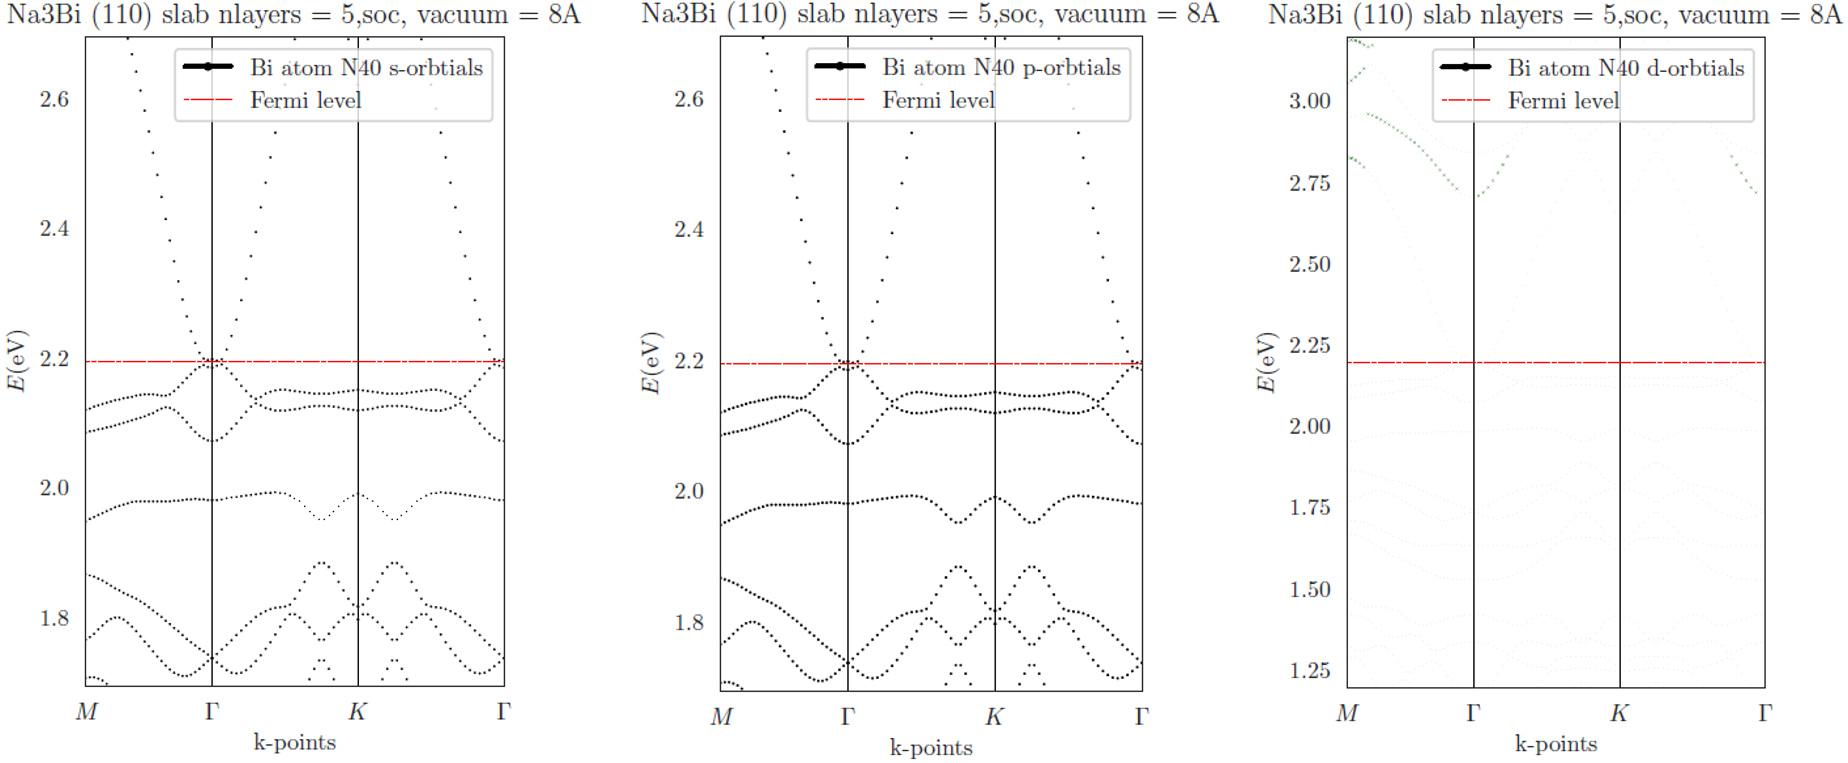
\includegraphics[scale=0.5]{Na3Bi_110_nlayer5_vac8_fatbands_Bi_N40}

\caption{\label{fig:Na3Bi_110_nlayer5_vac8_fatbands_Bi_N40} Fat band plots showing the contributions of Bismuth's orbitals on the band plot of 5 layer Na$_3$Bi in an 8A vacuum.}

\end{figure}


In Figure \ref{fig:Na3Bi_110_nlayer5_vac8_fatbands_Bi_N40} we plot the contributions of Bismuth's on the band structure for Na$_{3}$Bi. The Bi atom, labeled as atom number 40,  is located on the top surface of the Na$_{3}$Bi slab. Bismuth's p-orbtials contribute the most to the band plot, followed by its s-orbitals. The d-orbitals contribute the least.


\begin{figure}[H]

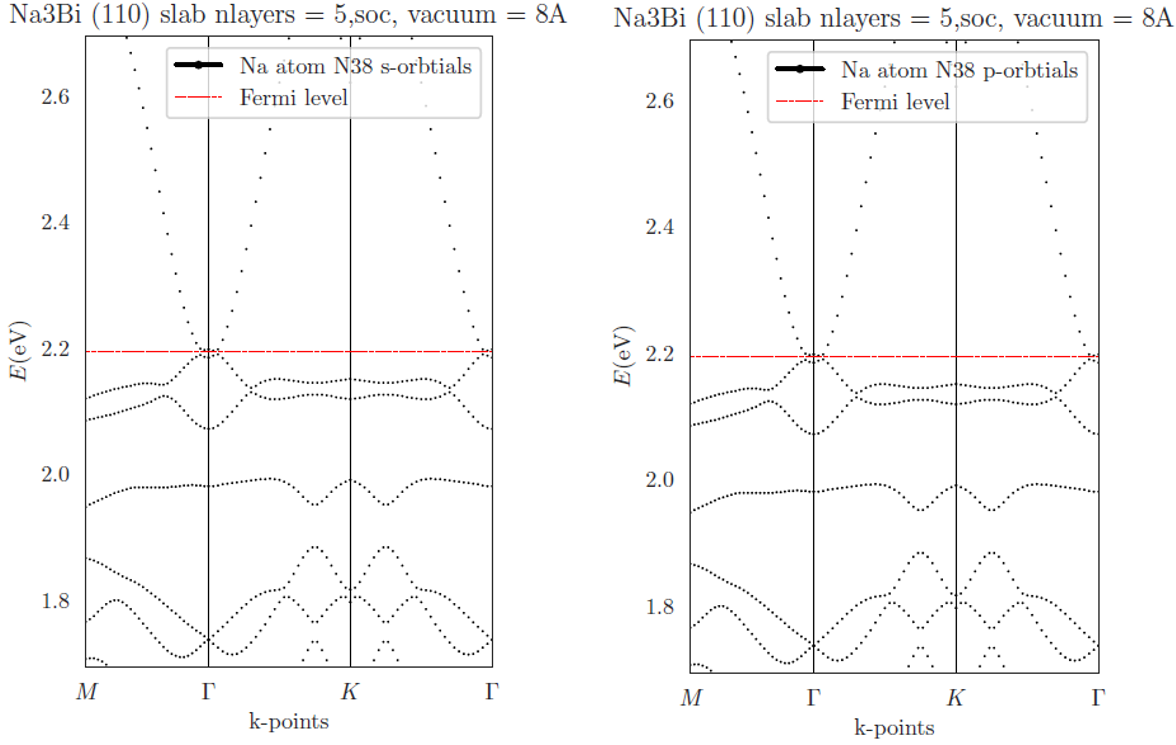
\includegraphics[scale=0.5]{Na3Bi_110_nlayer5_vac8_fatbands_Na38}

\caption{\label{fig:Na3Bi_110_nlayer5_vac8_fatbands_NaN38}The fat band plots of Sodium's orbitals on the band plots of 5 layer Na$_3$Bi in an 8A vacuum background.}

\end{figure}

In Figure \ref{fig:Na3Bi_110_nlayer5_vac8_fatbands_NaN38} we plot the contributions of Sodium's s and p orbitals to Na$_3$Bi's band plot. This Na atom is on the top surface of the Na3Bi slab.  It appears that both orbitals have equally relevant contributions to Na$_{3}$Bi's band plot.



%Na3Bi slab modulus behavior.
\subsection{Behavior of 5 layer Na$_{3}$Bi's wavefunctions.}

\begin{figure}[H]

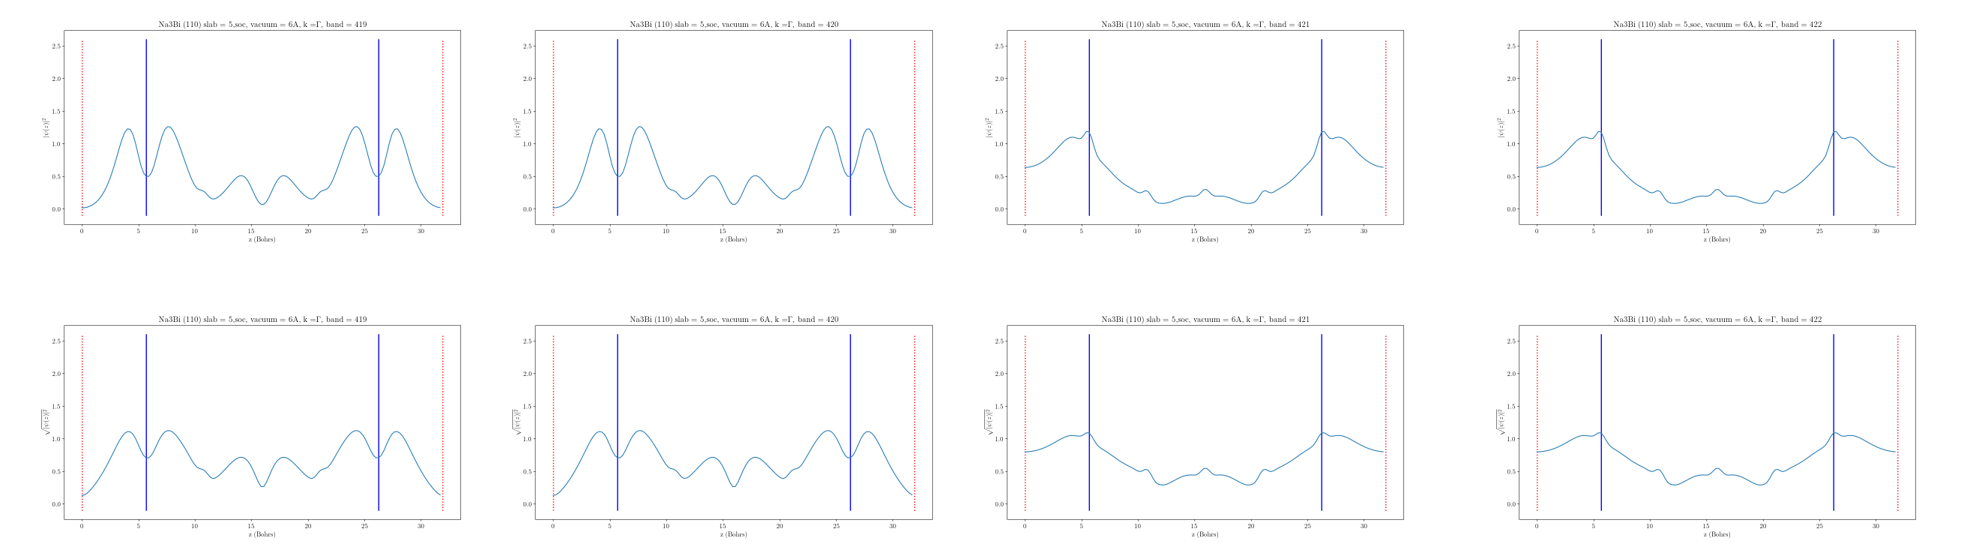
\includegraphics[scale=0.5]{Na3Bi_nlayer_5_vac6A_wavefunctions}

\caption{\label{fig:Na3Bi_nlayer_5_vac6A_wavefunctions}Modulus squared and modulus of bands closest to the Fermi level of 5 layer Na$_3$Bi surrounded by a 6A vacuum.}

\end{figure}


In Figure \ref{fig:Na3Bi_nlayer_5_vac6A_wavefunctions} we have plotted the modulus squared and modulus of the wavefunctions corresponding to bands 419-422, which are the bands closest to the Fermi level near the $\Gamma$ point.  The blue vertical lines denote the top and bottom surfaces of the Na$_{3}$Bi structure, while the red dotted lines denote the boundaries of the entire structure (which includes the vacuum layer). We see that the modulus squared plots for bands 419 and 420 have relative minima at the top and bottom surfaces.  However, just above and below these surfaces there are moduli maxima.  The same behavior is observed for their moduli.The bands 421 and 422 have maxima modulus squared and moduli values at the top and bottom surfaces.  Their squared moduli and moduli have greater values near these surfaces than in the bulk of Na$_3$Bi.  
\end{comment}

\section{Proposals.}

Can we find topological states in a heterostructure of an insulator and topological Dirac semimetal KTaO$_3$/Na$_3$Bi? If we cannot find topological states from this heterostructure, we can discuss why they cannot be found in such a heterostructure combination.  Perhaps we can figure out the behavior of the surface states in the insulator by studying the spin texture behavior of the surface states.   

How do surface states of a type-I Weyl semimetal such as TaAs interact with those of Na$_3$Bi in a heterostructure of the two? Recall that a Weyl semimetal has surface states which are ensured via the bulk-boundary correspondence and non-zero Chern number of the Weyl points.  This is in contrast to Dirac semimetals whose surface states which do not follow this correspondence.  

How do surface states of a type-II Weyl semimetal such as WTe$_2$ interact with those of Na$_3$Bi in a heterostructure of the two? A type-II Weyl semimetal has its Weyl cone tilted relative to the Fermi level such that the electron and hole pockets are intersected by the Fermi level.  How do the interactions between surface states in this heterostructure differ from the case of a type-I Weyl semimetal and Na$_3$Bi heterostructure?   

In heterostructures comprised of a ferromagnetic or antiferromangetic material and Na$_3$Bi, are the spin orbit torques affected by the presence of both gapless bulk and surface states?  

Is the out-of-plane spin accumulation, which is usually affected by the bulk states, have contributions from Na$_3$Bi's  Fermi arc states?





\begin{comment}
%Aluminum on Na3Bi heterostructure.
\subsection{Aluminum on Na$_3$Bi heterostructure data.}

\begin{itemize}

\item We want to investigate the fate of the Na3Bi surface states when Na$_3$Bi layers are stacked on Aluminum (Al) layers. 
\item We want to answer whether any hybridization occurs between the Na$_3$Bi surface states and the Al metallic states. If so, does this produce topological states?
\item We also want to observe how far the spin texture characterizing the Na$_3$Bi surface states penetrate into the Al surface. 
\item Since Na$_3$Bi and Al have distinct crystal structures, the former has a hexagonal P63/mmc phase crystal structure while the latter has a face-centered cubic crystal structure, they need to be stacked along certain orientations to minimize the lattice mismatch between both structures. 
\item Based on information from the Materials Project website, we orientate Al along the (111) direction on Na$_3$Bi, which is along the (110) direction.

\end{itemize}

%Band structure plot and electronic density of states for 1Al/3_Na3Bi heterostructure. 
\begin{figure}[H]

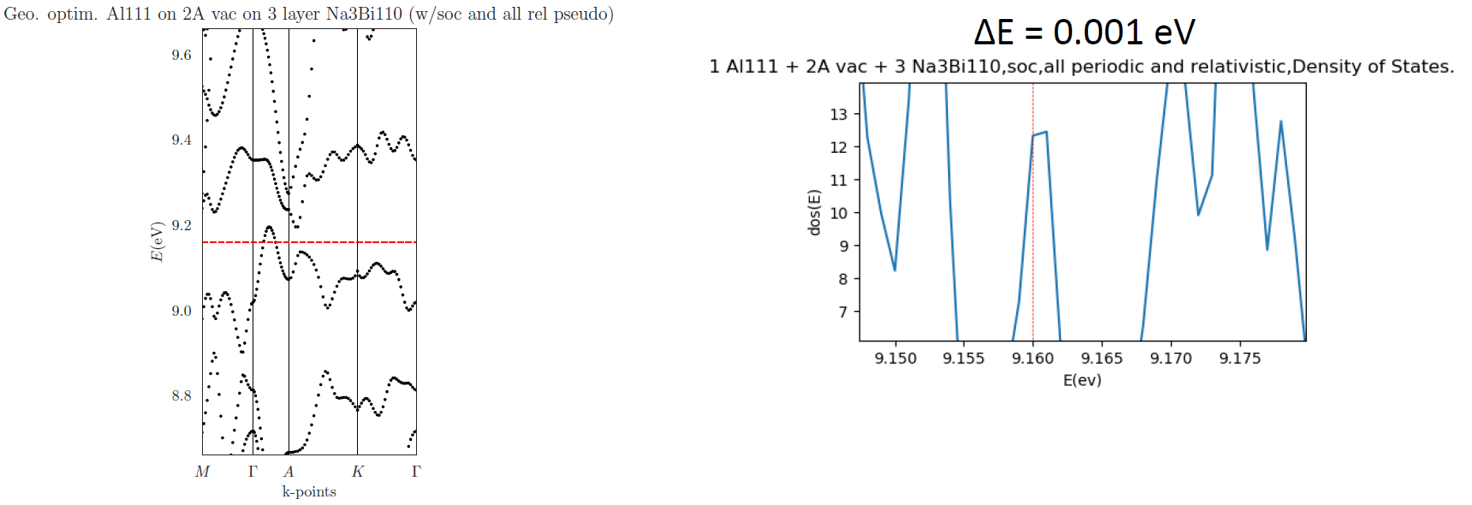
\includegraphics[scale=0.8]{Al111_on_Na3Bi_bandplot&DOS}\caption{\label{fig:1Al+3Na3Bi bandplot =000026 DOS.}Band structure plot and
electronic density of states for geometrically optimized Al/Na$_3$Bi heterostructure.}

\end{figure}


\begin{itemize}
\item We studied a single layer Al (111) on three layers of Na$_3$Bi (110) which were initially separated by 2A.  
\item We then perform a geometric relaxation calculation on this heterostructure.  It involves finding the optimal positions of the atoms in the heterostructure as well as the optimal cell of this structure.  
\item These optimizations are realized when the total energy and all components of the forces acting acting on all the atoms are below certain thresholds.
\item Figure \ref{fig:1Al+3Na3Bi bandplot =000026 DOS.} shows the band plot and electronic density of states for the geometrically relaxed heterostructure consisting of a single layer Al (111) on three layers of Na$_3$Bi (110).   
\item We observe this heterostructure is metallic since the Fermi level, indicated by the red dashed line, intersects a band with no finite energy gap immediately above the Fermi level which separates the filled and unfilled electronic states.
\item We find the same conclusion if we study the density of electronic states. This quantity signifies the number of available electronic states per unit energy per unit volume. We see above that there is a non-zero density of states around the Fermi level. 

\end{itemize}




%Modulus squared and modulus of wavefunctions of bands nearest the Fermi level at \Gamma. for the heterostructure. 
\begin{figure}[H]

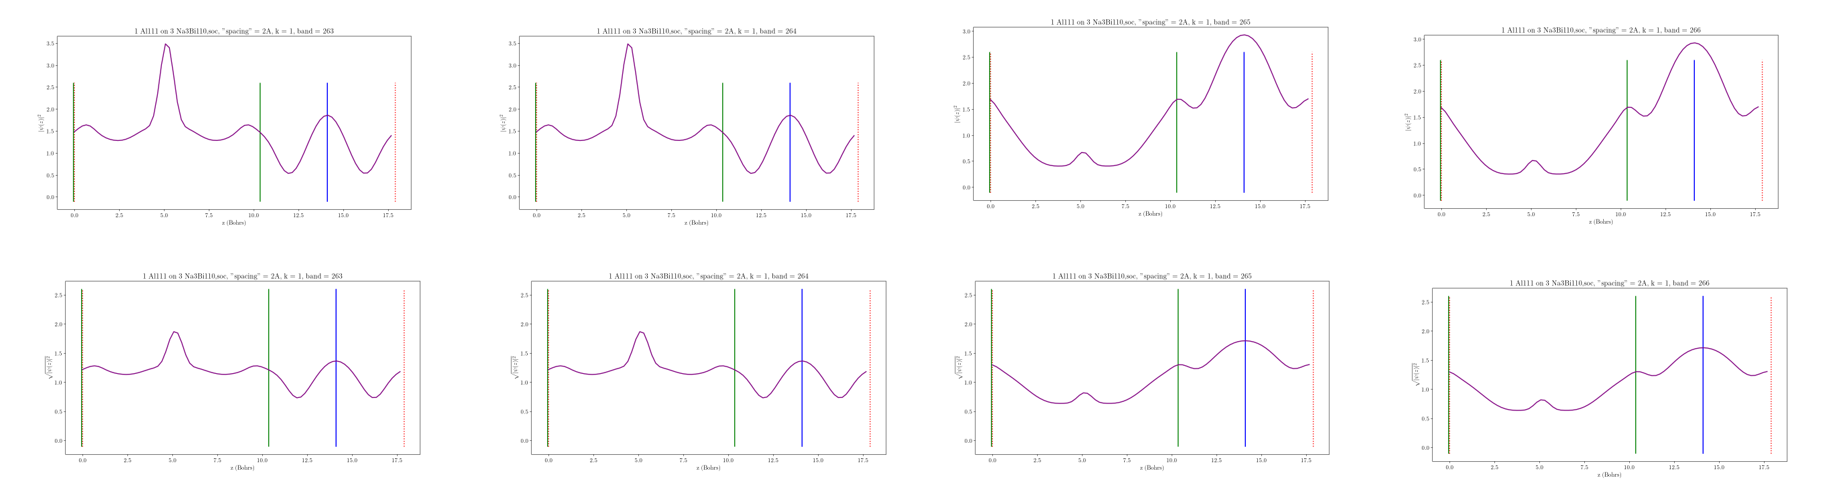
\includegraphics[scale=0.6]{Al111_on_Na3Bi_wavefunctions}\caption{\label{fig:Modulus squared and modulus of bands}Modulus squared and
modulus of bands closest to the Fermi level.}

\end{figure}



\begin{itemize}
\item Our heterostructure resides in $3+1$ dimensions.  The z-direction has open boundary conditions, while periodic boundary conditions are applied in the x and y directions.
\item Figure \ref{fig:Modulus squared and modulus of bands} shows the behavior of the modulus squared and modulus $\left|\psi\left(z\right)\right|^{2}$ and $\sqrt{\left|\psi\left(z\right)\right|^{2}}$ of the wavefunctions corresponding to bands $263 - 266$.  These are the the bands closest to the Fermi level at $\Gamma$. The valence bands correspond to bands 263 and 264, while the conduction bands are bands 265 and 266.
\item The green and blue vertical lines denote the boundaries of the Na$_3$Bi and Al layers, respectively, while the red dashed lines are the boundaries of the structure which includes any space between the Na$_3$Bi and Al layers.
\item The valence bands have a modulus that is peaked around the center of the Na$_3$Bi system. This modulus dips in the region between the Na$_3$Bi and Al layers and between the Al layers and the upper structure boundary.  
\item A relative maximum of the modulus that appears at the single Al layer.
\item The conduction bands' squared moduli behave completely different; their maxima appears around the Al layer.
\item Relative maxima in the squared moduli occur at the surfaces of the Na$_3$Bi structure.
Between the Na$_3$Bi and Al structure, the squared moduli are not at all minimum. 
\item Conduction bands have a minimum around the center of the Na$_3$Bi structure. 
\item As for the analogous moduli plots, there is not much to say for them: they appear to follow the trends of the modulus squared plots.
\item The moduli plots indicate there is no hybridization between the Na$_3$Bi surface states and the Al states. 
\item However, we only have a single Al layer present. We want to increase number of Al layers in the heterostructure to observe any changes in the modulus and modulus squared plots as well as the band plots.
\item Additionally, we are attempting to find the behavior of the surface states in a heterostructure consisting of Na$_3$Bi and KTaO$_3$, the latter being an insulator.
\end{itemize}

\end{comment}

\printbibliography

\end{document}
